\documentclass{kththesis}

\usepackage{csquotes} % Recommended by biblatex
\usepackage[style=numeric,sorting=none,backend=biber]{biblatex}
\usepackage{amssymb}
\usepackage{hyperref}
\usepackage{amsthm}
\usepackage{amsmath}
\usepackage{listings}
\usepackage{minted}
\usepackage{tcolorbox}

\usepackage{etoolbox}%Used? 


\newtheorem{definition}{Definition}

%T: Set up toc links
\hypersetup{
    linktoc=all,     %set to all if you want both sections and subsections linked
    linkcolor=black,  %choose some color if you want links to stand out
}

\addbibresource{references.bib} % The file containing our references, in BibTeX format

\title{Alternating Control Flow Graph Reconstruction Using Constant Propagation and Directed Symbolic Execution}
\alttitle{Alternaterande kontrollflödesgrafsrekonstruktion genom propagerande av konstanter och riktad symbolisk exekvering}
\author{Thomas Peterson}
\email{thpeter@kth.se}
\supervisor{Roberto Guanciale} 
\examiner{Mads Dam}
\programme{Master in Computer Science}
\school{School of Electrical Engineering and Computer Science}
\date{\today}

%-----Custom Commands-----
\newcommand{\MONTH}{%
  \ifcase\the\month
  \or January % 1
  \or February % 2
  \or March % 3
  \or April % 4
  \or May % 5
  \or June % 6
  \or July % 7
  \or August % 8
  \or September % 9
  \or October % 10
  \or November % 11
  \or December % 12
  \fi}
  
\renewcommand{\it}[1]{\textit{#1}}

\renewcommand\fcolorbox[4][]{\textcolor{cyan}{\strut#4}} %Remove minted error boxes

\lstset{columns=fullflexible,
        mathescape=true,
        literate=
               {<-}{$\leftarrow{}$}{1},
        tabsize=4,
        frame = single,
}
        
\lstdefinestyle{top}{
  float=tp,
  floatplacement=tbp,
  abovecaptionskip=-1pt
}

% Uncomment the next line to include cover generated at https://intra.kth.se/kth-cover?l=en
% \kthcover{kth-cover.pdf}


%---Notes---
%A conscientiously written scientific report in Swedish or English where the problem is introduced, different methods for the solution are discussed, the method chosen is presented, the solution and the results are described and the results are analyzed

%---Before Handing in the Report--

%Content checklist: https://www.kth.se/social/group/examensarbete-vid-cs/page/degree-project-checklist/

%Formalitiees checklist: https://www.kth.se/social/group/examensarbete-vid-cs/page/formalities-checklist/

%Read the opposition documents: https://www.kth.se/social/group/examensarbete-vid-cs/page/public-discussion-and-examination/

%Check that all sources look good! And try to double check correctness!
%---------------------------------
%---TODO---
%Ensure abbreviations(like CFG) are introduced with the first occurrence of the notion
%Ensure consistent usage of intel or AT&T x86 syntax
%---------------------------------
%---Potential things to add---
% Info on stripped vs non-stripped binaries
%---------------------------------

\begin{document}

% Frontmatter includes the titlepage, abstracts and table-of-contents
\frontmatter

\titlepage

\begin{abstract}
%\\ \\
%\textbf{Keywords}\\
%Binary analysis, Control flow reconstruction, concolic execution
\end{abstract}


\begin{otherlanguage}{swedish}
  \begin{abstract}
    ...
  \end{abstract}
\end{otherlanguage}
%\clearpage
%\section*{Acknowledgement}
%I would like to thank my supervisor Roberto Guanciale, for his feedback and guiding throughout the research and writing of this report. 
%\\ \\
%Thank you! 
%\\ \\ \\ \\
%Stockholm, \MONTH \the\year
%\\ \\
%\it{Thomas Peterson}

\tableofcontents
\thispagestyle{empty}

\clearpage
\thispagestyle{empty}
\section*{Abbreviations}
\textbf{BBG:} Basic Block Graph\\
\textbf{CFG:} Control Flow Graph\\
\textbf{CFA:} Control Flow automaton\\
\textbf{IR:} Intermediate Representation\\
\textbf{Jakstab:} \textbf{Ja}va tool\textbf{k}it for \textbf{sta}tic analysis of \textbf{b}inaries\\

\clearpage
\thispagestyle{empty}
\section*{Glossary}
\textbf{Direct Jump:} A jump instruction which jumps to an explicit address.\\
\textbf{CFG:} A BBG or a CFA.\\
\textbf{Indirect Jump:} A jump instruction which jumps to an address located in a register or a memory location.\\
\textbf{Jump table:} A data structure which sometimes results from switch cases and frequently leads to indirect jumps. \\
%\textbf{Transpilation:} The act of translating a binary program into its equivalent IL program\\

% Mainmatter is where the actual contents of the thesis goes
\mainmatter
\cleardoublepage
\pagenumbering{arabic}

%---INFO ABOUT CITATIONS---
%We use the \emph{biblatex} package to handle our references.  We therefore use the command \texttt{parencite} to get a reference in parenthesis, like this \parencite{heisenberg2015}.  It is also possible to include the author as part of the sentence using \texttt{textcite}, like talking about the work of \textcite{einstein2016}.

\chapter{Introduction}
%X The question is easy to identify, the project's purpose and objective are clear.
%X The problem (and the student's contribution) has defined limits, its relevance is justified and put in context
%
%Explain why we want to study the binary instead of the source code. Use example in WYSINWYX where memset was removed by compiler?
Software is normally not developed directly in assembler but indirectly in a higher-level programming language such as C. Before software can be used, its code must be compiled into machine-dependent assembly code, denoted as binary code. However, the compilation process can vary depending on many factors such as, for example, the type of compiler and the optimization level. Consequently, software written in a high-level language might have multiple binary representations, some of which might even be erroneous\cite{preciseCFG}. Thus, when analysing software, it might be incorrect to expect properties which hold in the source code to hold in the compiled binary. A prime example of this is xcodeGhost.
\\ \\
Xcode is an application development framework for building IOS applications, developed by Apple\cite{Xcode}. In china, network speeds to apple's servers could sometimes be very slow and IOS developers thus commonly shared copys of Xcode installers through other hosting services\cite{XcodeGhost}. In mid-2015, malicious copys of xcode installers began circulating. These installers, known as XcodeGhost\cite{XcodeGhost}, appeared to behave identically to the legitimate framework. However, during compile time, the framework would inject malware into the application. Thus, the infected developers would unintentionally create infected applications. 
\\ \\
XcodeGhost was the first compiler malware in OS X and the first instance of the IOS App Store deploying a large amount of trojanized applications\cite{XcodeGhost}\cite{XcodeGhostFireEye}. It successfully infected a large amount of IOS applications, of which only two were immediately confirmed to succesfully have passed apples code review and been submitted to the App Store for public download\cite{XcodeGhost}. Later, the cyber sercurity company FireEye conducted an investigation where they determined that more than 4000 different IOS apps had been infected, passed Apple's code reviews and been available for public download. The infected apps stole user data and could accept remote commands from a command and control server\cite{XcodeGhostFireEye}, potentially exploiting the infected devices as bots to create a botnet.
\\ \\
The XcodeGhost malware clearly motivates the study of binary-level analysis rather than source code analysis as source code analysis would not have been able to find anything wrong with the applications. Moreover, another incentive to binary-level analysis is that source code is often unavailable as many commercial off-the-shelf (COTS) software and third-party libraries are distributed only in binary form\cite{preciseCFG}.
\\ \\
As binary code is more verbose than high-level code, it is infeasible to manually analyze large binaries. Consequently, many binary analysis platforms have been created to automate binary analyses\cite{BitBlaze}\cite{BAP}\cite{TrABin}\cite{CodeSurfer}. Binary analysis has thus become a broad field with many different applications. It might, for example, be used for program verification\cite{TrABin}, exploit generation\cite{angr} or detection of memory management errors\cite{valgrind}. Further, Binary analysis can be useful even in situations where the source code is available. Such situations can, for example, occur when the compiler is not part of the trusted computing base and one would like to empirically establish that properties of the source code still holds in its corresponding binary.
\section{Problem Statement}
One fundamental obstacle when performing binary analysis is the lack of precise control flow information. There are already many existing approaches to control flow reconstruction. These can be categorized as static or dynamic techniques. Static techniques studies the binary without performing concrete executions. Instead, they reason about the binary in an abstract manner. Dynamic techniques, on the other hand, concretely executes the binary with different inputs with the intention of triggering different control flow paths. 
\\ \\ 
Static analysis often suffers from problems stemming from indirect jump instructions. These are jump instructions where the processor is instructed to jump to a value stored in a register or memory location rather than an explicit address encoded in the instruction. As it is very expensive to keep track of all memory and register content, it is expensive to calculate the target location of such jumps. Consequently, many static analysis tools resort to approximations which are not always precise.
\\ \\
The main objective of this thesis is to study how the precision of CFG reconstruction can be improved in the context of alternating over/under-approximation approaches. More specifically, it is studied how indirect jump resolution can be improved by using under-approximation when over-approximation can not deduce a finite set of possible targets. The thesis is limited to x86 binaries and primarily targets binaries without additional source code information.
\\ \\
In this thesis, we investigate an approach based on alternating over/under-approximation inspired from previous work\cite{alternating}. Furthermore, the constant propagation used for over-approximation is based on previous work by Kinder et al\cite{Jakstab}. Finally, the under-approximation techniques are inspired by white-box fuzzing techniques.
%"The automatic test generation will be conducted through white-box fuzzing and the over-approximation will use constant propagation as it scales well to large binaries\cite{Jakstab}. The goal will be to study to what extent precision and coverage can be improved if one were to use white-box fuzzing techniques instead of random fuzzing techniques in the context of over/under-approximation approaches. The algorithm will resort to under-approximation only when the over-approximation can not determine a finite amount of possible jump targets. In the case where both the under and over-approximation can not determine the targets, the branch will be assumed to be non-feasible. This has the benefit of avoiding to create a degenerate CFG by adding an edge from the branch location to every possibile location in the program."

\section{Related Work}
%Goal: What has been done? What hasn't been done? What can I contribute with? Why would that be important? 
%Codesurfer? BitBlaze?
There have been many approaches to control flow graph reconstruction through the last couple of centuries. However, to our best knowledge, no one has succeeded in developing an algorithm that can construct the ideal CFG for an arbitrary binary. There are however many platforms that can create approximations of the ideal CFG. The approach described in this paper differs from others in the sense that it gives up on properties such as soundness and completeness to completely focus on precision. 
\\ \\
Angr\cite{angr} is a state-of-the art binary analysis platform for exploit generation. It was created as part of the DARPA challenge and was used by the team Shellphish. It is heaviliy modularized and has borrowed the intermediate language VEX from valgrind, a platform which focuses on finding memory leaks in programs. The angr project contains two CFG reconstruction algorithms named \textit{CFGAccurate} and \textit{CFGFast}. The \textit{CFGFast} is a purely static analysis algorithm while \textit{CFGAccurate} leverages dynamic analysis through its dynamic symbolic execution engine. 
\\ \\
The \textit{CFGAccurate} algorithm uses techniques such as forced execution, backwards slicing, symbolic execution and value set analysis to create an accurate representation of the CFG. The angr CFGAccurate algorithm is similar to our approach in the sense that it does not provide any soundness or completeness guarantees. However, a difference is that our approach represents the CFG as a CFA rather than a BBG and thus might be able to create more expressive control flow graphs. Additionally, the approach presented in this thesis works with different abstract domains.
\\ \\
Another approach is to use the forced execution technique presented by Xu et al\cite{preciseCFG}. This technique performs pure under-approximation through manipulation of concrete executions and distinguishes itself from many other approaches by working directly on the binary rather than using an intermediate representation of the binary. The presented algorithm executes the program on a selected starting input and records snapshot of the program state at every jump statement. Once the initial concrete execution finishes, the program state is reset to one of the earlier snapshots and resumed. 
\\ \\
This process of restoring snapshots and resuming execution continues until every possible execution has been performed. However, the algorithm is not complete since it can force execution of infeasible edges. If one would exclude the infeasible edges added through the forced execution of infeasible branch targets, their results would, in theory, be an ideal CFG. However, due to several problems such as for example, infinite loops, their algorithm can not be guaranteed to finish in finite time. Consequently, they adapt the algorithm to be more practical at the expense of the guarantee of exploring every possible CFG edge. 
\\ \\
Another approach was introduced by De Sutter et al\cite{staticOfInd}. In their paper, they coin the terms hell node and hell edges. The paper defines a hell node as a node which represents all possible targets of an unresolved indirect jump. Further, they define hell edges to be edges connected to the hell node. They proceed with their analysis by noting that indirect jumps have five major sources: switch-statements implemented with a table lookup and indirect jump, exception handling, goto statements to pointer assigned labels as well as the use of procedure pointers and dynamic method invocation in object oriented languages. They are able to resolve all indirect jumps of switch cases by trying to match program slices of the part of the program calculating the jump target, with common instruction sequences for switches. For all other jumps they try to obtain the targets using constant propagation.
\\ \\
An alternative to program slicing and constant propagation is to use abstract interpretation as in the CFG reconstruction algorithm developed by Bogdan Mihaila\parencite{CFGFromPowerPC}. This algorithm soundly over-approximates the control flow in a top-down manner. Their analysis heavily focuses on resolving indirect jumps stemming from jump tables. They define an interval domain and a set domain using abstract interpretation. These domains are then used to over-approximate the targets of the indirect jumps. A similarity between their work and ours is that they represents the CFG as a CFA rather than a BBG. Conversely, a difference is that they assume data structures in the binary to conform to source-code-level data structures, which we do not. 
\\ \\ 
Among the static analysis approaches there are also approaches which do not rely on abstract domains. On such approach was presented by Reinbacher et al. In their approach, they linearly disassemble the binary into instructions that are then grouped into basic blocks. Afterwards, they express the semantics of each basic block using boolean logic. Thereafter, each basic block is converted to its corresponding CNF form using Tseitin conversion. They then apply forward and backward traversal to generate pre and post conditions for the binary blocks. The backward traversal is limited to k basic blocks, where k is a tunable parameter. Consequently, it is possible to tune to what extent previous blocks should be used when calculating pre and post conditions for a basic block. Furthermore, this offers a trade-off between speed and precision which can be useful in various applications which require less of one or the other.
\\ \\
As their calculations of pre and postconditions are conducted through the usage of a sat-solver, an advantage of their approach is that the performance of the algorithm will benefit from performance increases of sat-solvers in the future. Finally, the results of their empirical experiments indicate that the forward-backward analysis introduced can, not only be more precise, but actually also be faster than pure forward analysis. The authors concluded that this is because the value sets propagated around the program tend to be smaller.
\\ \\
A state of the art platform for static analysis and control flow reconstruction is Jakstab\cite{JakstabGit}, developed by Kinder et al\cite{Jakstab}. This platform uses abstract interpretation to, under very general assumptions, simultaneously determine the CFG and data flow of a binary. This is conducted by using an intermediate language, on-demand disassembly, an extended version of the classic worklist algorithm and bounded address tracking. Bounded Address Tracking is a highly precise abstract domain that models registers and memory locations as both pointers and integer values. The CFG generated is a sound over-approximation of the true CFG and is represented by a Control Flow automaton. Consequently, it can distinguish between different states with the same IP value.
\\ \\
In a later work, Kindner et al extended Jakstab to work with alternating over/under-approximation\cite{alternating}. In this work, they created an abstract domain representing the combination of their over and under-approximation approaches. For the over-approximation they used bounded address tracking of the Jakstab platform. For the under-approximation, they extended Jakstab to support replaying execution traces. The execution traces were recorded by executing the binary in qemu and tracing the control flow. The targets of branches which could not be approximated through over-approximation, could then be under-approximated with the traces. 
\\ \\
In this thesis, the Jakstab tool is extended by using symbolic execution techniques for the under-approximation part of the alternating over/under-approximation approach. More specifically, directed symbolic execution is applied to determine path constraints to reach specific unresolved branches. These path constraints are then used to generate input that would lead a concrete execution to the unresolved jump. Then, a concrete execution with this input is performed, the jump target is recorded and the approximated CFG updated. This approach of directed symbolic execution has the benefit of avoiding the path explosion problem of naive symbolic execution approaches. Additionally, it can potentially ensure that unresolved branches will eventually be resolved, contrary to the trace recording approach with random input.
%"The CodeSurfer/x86 project originally suffered from the problem that every analysis in principle had to implement an abstract transformer for each x86 assembly instruction, which in practice led to omitting large parts of the instruction set" (static analysis of x86 binaries)

\section{Outline}
The outline of the thesis is as follows. In chapter \ref{chap:background} a theoretical background is provided. This background serves as a foundation for understanding the remaining parts of the thesis. In chapter \ref{chap:methodlogy} the degree project methodology is presented and in chapter \ref{chap:results} the results are illustrated and described. Thereafter, a summary of the thesis is provided and discussions are made regarding further possible work in chapter \ref{chap:discussionAndConclusions}.
 
\chapter{Theoretical Background}\label{chap:background}
%X The student displays knowledge of theoretical background and previous related work (significant literature is mentioned and relevant material is used).
%X The background is coherent and relevant.
This chapter provides a theoretical background describing the theory needed to understand the remaining parts of the thesis.
% Should probably explain Application binary interface (ABI)
%Mention switchs and jump tables? 

%http://ee.usc.edu/~redekopp/cs356/slides/CS356Unit5_x86_Control.pdf
%Jump types
%Flags (ZF e.t.c)
%Comparision instructions
%Good reference: https://software.intel.com/sites/default/files/managed/39/c5/325462-sdm-vol-1-2abcd-3abcd.pdf 
%TODO: Check if instructions are correct (relative/absolute)
\section{Control Flow in the x86 Architecture}
Assembly instructions can be categorized into three possible control flow transitions. The first type is fall-through instructions\cite{CFGFromPowerPC}. These instructions are instructions which, after being executed, simply increments the IP the size of the instruction. Consequently, the execution continues with the instruction immediately after the fall-through instruction. Instructions which do not classify as fall-through instructions are denoted as jump instructions. 
\\ \\
The last two types are direct and indirect jumps. Jumps are instructions which transfers the flow of execution by changing the instruction pointer register by a specified value. The difference between a direct and and indirect jump is that a direct jump is a jump to an explicit address whereas an indirect jump is a jump to an address stored in a register or a location in RAM. 
\\ \\
Furthermore, jumps can also be categorized into conditional and unconditional jumps. Unconditional jumps are jumps that always jump to a specified location. Conversely, conditional jumps are jumps that only jump to a specified location if a certain condition holds. Otherwise, the instruction pointer is simply incremented by the instruction size to instruct the CPU to execute the next instruction. 
\\ \\
The following example will explain the difference between conditional and unconditional jumps as well as direct and indirect jumps, using x86 instructions. X86 instructions can be represented with Intel or AT\&T syntax. In this thesis, examples uses the Intel syntax.
\\ \\ 
Table \ref{tab:jumps} provides examples illustrating the difference between conditional and unconditional jump instructions as as well as direct and indirect jump instructions. The instruction \textit{jmp 0x00401078}, located in the the top-left cell of the table, is an example of an direct and unconditional jump. It is unconditional since it uses the \textit{jmp} instruction which instructs the CPU to jump to the specified address unconditionally. Furthermore, it is direct since the address \textit{0x00401078} is specified explicitly. Note that the address \textit{0x00401078} is arbitrary chosen for the sake of illustration and does not have any special meaning.

\begin{table}[ht]
\centering
\begin{tabular}{lllll}
\cline{1-3}
\multicolumn{1}{|l|}{\textbf{}}              & \multicolumn{1}{l|}{\textbf{Direct}} & \multicolumn{1}{l|}{\textbf{Indirect}} &  &  \\ \cline{1-3}
\multicolumn{1}{|l|}{\textbf{Unconditional}} & \multicolumn{1}{l|}{jmp 0x00401078}    & \multicolumn{1}{l|}{jmp eax}           &  &  \\ \cline{1-3}
\multicolumn{1}{|l|}{\textbf{Conditional}}   & \multicolumn{1}{l|}{je 0x00401078}     & \multicolumn{1}{l|}{je eax}            &  &  \\ \cline{1-3}
                                             &                                      &                                        &  &
\end{tabular}
\caption{A table illustrating the difference between unconditional and conditional jump instructions as well as direct and indirect jump instructions.}
\label{tab:jumps}
\end{table}
\noindent
The instruction \textit{jmp eax}, located in the the top-right cell of the table, is an example of an indirect and unconditional jump. Similarly to the instruction in the top-left cell, it is unconditional since it uses the \textit{jmp} operand which instructs the CPU to jump to the specified address unconditionally. Further, it is indirect since it is instructed to jump to the address located in the register \textit{eax}.
\\ \\
The bottom-most row contains conditional jump instructions. These are instructions that executes a jump only if a specific condition is satisfied. For example, the instruction \textit{je 0x00401078} in the bottom-left cell is conditional since it only jumps if a previous compare instruction compared two values that were equal. Furthermore, this instruction is a direct instruction since it jumps to the explicitly specified address \textit{0x00401078}.
\\ \\
Finally, the bottom-right cell contains an instruction which is a conditional indirect jump. This can, similarly to previous instructions, be seen through its usage of the operand \textit{je} which jumps only on equality between two values and the implicitly specified jump location through the register eax.
\\ \\
%SF - 1 if MSB (aka sign bit) of result = 1
%PF - 1 if Parity of Least significant byte is even
%CF - 1 if unsigned op2 > unsigned op1
%OF - 1 if sign bit of OP1 != sign bit of result
%AF - 1 if Carry in the low nibble of result
Before a conditional jump is executed, the CPU usually executes some sort of compare instruction. In x86, a common compare instruction is \textit{cmp} which takes two arguments. It subtracts the first argument from the second and sets a set of register flags according to the result of the subtraction. More specifically, the \textit{cmp} instruction modifies the \textit{SF}, \textit{ZF}, \textit{PF}, \textit{CF}, \textit{OF} and \textit{AF} flags. The \textit{SF} flag is set if the difference is negative and the \textit{ZF} flag is set if the difference is exactly 0.
\\ \\
Furthermore, the \textit{PF} flag is set if the difference has an even number of set bits and the \textit{CF} flag is set if the second argument would be greater than the first in an unsigned comparision. Finally, the \textit{OF} flag is set if the sign bit of the first argument does not equal the sign bit of the result and the \textit{AF} flag is set if the four least significant bits of the results did not result in a carry. When executing one of the \textit{je} instruction in the above examples, the CPU would check that the \textit{ZF} flag is set before performing a jump to the specified location since the \textit{je} instruction only jumps on equality.
\\ \\
Apart from jump instructions, there are also \textit{call} instructions which can alter the control flow of a program. Normally, \textit{call} instructions are used to invoke a procedure. Initially, the program pushes it's arguments to the stack (Or alternatively puts them in registers). Thereafter, the program executes the call instruction, which is a push of a return address to the stack and an unconditional jump to the start of the procedure. At the end of the proceddure, there is usually a return instruction \textit{RET}. The \textit{RET} instruction pops the stack to obtain the return address that was pushed by the call instruction. Then, it instructs the CPU to perform and unconditional jump to the obtained return address. 
\\ \\ 
In this work, the theoretical framework of the over-approximation treats \textit{call} instructions in the same way as unconditional \textit{jmp} instructions.

%Control flow graph have one entry node but might have multiple exit nodes. Can also have multiple input nodes if one only looks at part of the program. For example, if one would like to reconstruct the CFG of a funciton, this function might be called from multiple positions in the program.
%"They explain that indirect jumps have five major sources: switch-statements implemented with a table lookup and indirect jump, exception handling, goto statements to pointer assigned labels and use of procedure pointers and dynamic method invocation in object oriented languages." lit stud
%Background of cfg, why use them
%\\ \\
%Chicken and egg problem between Data flow analysis and control flow graph reconstruction.
%\\ \\
%
%intra-procedural
%inter-procedural
%\\ \\
\section{Control Flow Graphs}
The control flow of a program is defined as what instructions are executed in what order. A Control Flow Graph(CFG) is a directed graph which illustrates the control flow of a program. This graph is usually represented by either a Basic Block Graph or a Control Flow Automaton.
\\ \\
A Basic Block Graph(BBG) is defined as a directed graph G = (V,E) where V is a set of nodes representing blocks of instructions, called basic blocks, and E is a set of edges representing all the possible transitions between the basic blocks. Each basic block consists of a set of fall-through instructions and at most one jump instruction at the end the block. As all fall-through instruction are contained in basic blocks, each edge in the CFG corresponds to either a direct or an indirect jump.
\\ \\ 
Denote by $Stmt$ the set of basic and abstract statements. Further, denote by $L \in I_{32}$ the set of potential values of the instruction pointer. Then, a Control Flow Automaton(CFA) is defined as a tuple <$T,V,start,E$>, where $T \subseteq L$ is the set of program locations, $V$ is the set of registers, $start$ is an initial location such that $start \in T$ and $E$ is an edge relation $E \subseteq T \times Stmt \times T$. 
\\ \\
When a CFA is depicted as a graph, the nodes represent logical states $T \times V$ in the program and edges correspond to statements in the relation $E$. An advantage of CFA:s over BBG:s is that their nodes naturally correspond to program states and the edges corresponds to state transformations\cite{Jakstab}. Consequently, as a BBG can only represent connections between instructions, CFA:s can more accurately represent the control flow of a binary than BBG. 
\\ \\
To better understand this, consider the assembly code in figure \ref{fig:assembly}. The string "Hello World!" is stored in the data section of the binary and the text section contains the code for writing "Hello World!" to stdout ten times. The code contains the labels start, dec, print and quit as these can be used as jump targets for the jump instructions. Initially, the program sets the value of edi to 10 as this register is used to count how many times the string has been printed to stdout.
\\ \\
The program then compares $edi$ to 0 and jumps to \it{quits} if this holds. Then, it decrements $edi$ by 1 and fills the registers with values for performing a system call to write the string to stdout. The register $edx$ is set to the length of the string, $ecx$ to the address of the string, $ebx$ to the file descriptor of stdout and $eax$ to the opcode of the write instruction. After the write it jumps back to the compare instruction. to check if $edi$ is still more than 0. 
%See page 119 in jakstab thesis for pros and cons with cfa vs bbg
\begin{figure}[t]
    \centering
\begin{tcolorbox}
\begin{minted}[fontsize=\footnotesize]{gas}
SECTION .data
msg     db      'Hello World!', 0x0A

SECTION .text
start:
        mov edi,10  ;Set the edi register to 10
dec:
        cmp edi,0   ;Compare edi with 0
        je quit     ;Jump to quit if edi=0
print:
        dec edi     ;Decrement edi by 1
        mov edx, 13 ;Set edx to 13
        mov ecx, msg;Set ecx to the address of msg
        mov ebx, 1  ;Set ebx to 1
        mov eax, 4  ;Set eax to the opcode of write
        int 0x80    ;Perform the syscall
        jmp dec     ;Jump to dec
quit:
        mov ebx, 0  ;Set ebx to 0
        mov eax, 1  ;Set eax to the opcode of exit
        int 0x80    ;Perform the syscall
\end{minted}
\end{tcolorbox}
\caption{Assembly code of the example BBG and CFA graphs.}
    \label{fig:assembly}
\end{figure}


\begin{figure}[ht]
    \centering
    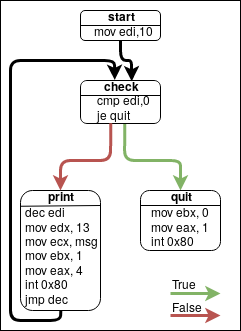
\includegraphics[scale=0.6]{Images/CFGExample.png}
    \caption{The BBG of the "Hello World!" Program. True and false branch conditions are illustrated with green and red arrows respectively.}
    \label{fig:HelloBBG}
\end{figure}
\clearpage
\noindent
The BBG of the hello-world program is illustrated in figure \ref{fig:HelloBBG}. There are multiple problems with the BBG. Firstly, from the BBG, it appears that a possible path could be \it{start}, \it{dec} and \it{quit}. However, this path is not possible in practice. Furthermore, from the BBG it is also not possible to tell if the program will ever terminate without studying the assembly code. This is because it appears that the program could execute \it{start} and then get stuck in an infinite loop between \it{check} and \it{print}.
\begin{figure}[th]
    \centering
    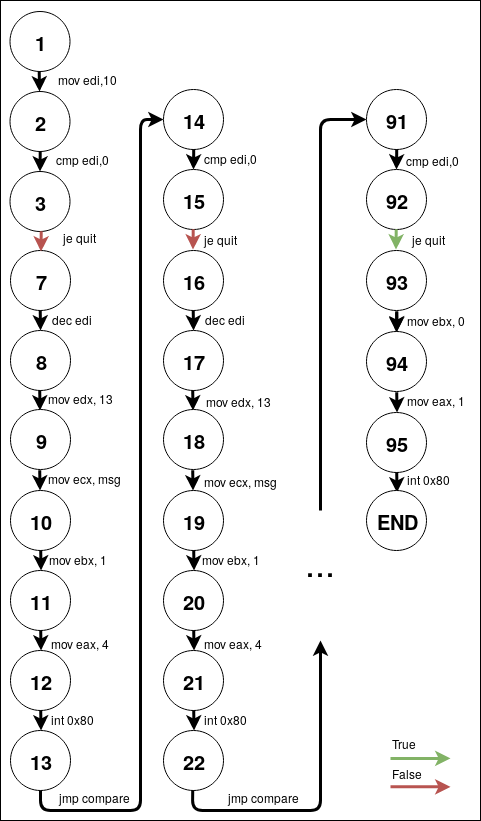
\includegraphics[scale=0.4]{Images/CFA.png}
    \caption{The CFA of the "Hello World!" Program. True and false branch conditions are illustrated with green and red arrows respectively.}
    \label{fig:HelloCFA}
\end{figure}
\noindent
\\
In the CFA of the hello-world program, which is depicted in figure \ref{fig:HelloCFA}, there is only one possible path. This is because a node is no longer a group of instructions but rather a set of register values which represent the state of the CPU. Consequently, state 2, 14 and 91 are distinct as they differ in the $edi$ value. More specifically, in this example, state 2, 14 and 91 correspond to $edi=10$, $edi=9$ and $edi=0$ respectively. Note, that conditional jump instructions does not have to correspond to two possible edges as the condition can be fully determined by the state. 
\\ \\
A problem with the usage of BBG:s when representing control flow is, for example, when conducting control flow integrity checks. When Control flow integrity checks are performed, the auditing software performing this checks uses information about what instructions can transfer control flow to which locations. It then audits executing programs to verify that all control flow transfers are performed according to these targets. If, however, a BBG is used, an attacker could enter a basic block from one edge and exit from an edge that shouldn't be feasible in practice when the entry edge was used. For example, if an attacker could manipulate the control flow of the hello world program so that it executed start, check and quit, this would be undetected by the control flow integrity checks. 
%Mention example of control flow integrity(A CFG overapproximates double function calls, thus, using control flow hijacking it is possible to jump somewhere it shouldn't be possible)
% Soundess + completness example in graph + Cascading loss of precision
\begin{figure}[t]
    \centering
    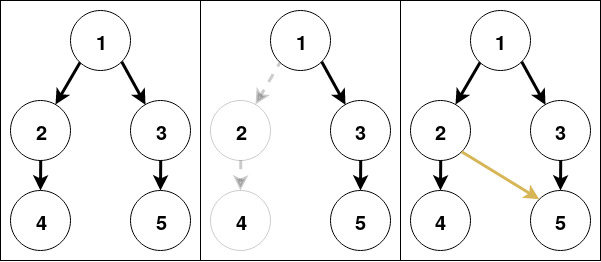
\includegraphics[scale=0.6]{Images/SoundCompleteGraph.png}
    \caption{An example of soundness and completeness in CFG:s. The left-most graph is the ideal CFG, the middle graph is a complete approximation of the ideal CFG and the right-most graph is a sound approximation of the ideal CFG. The transparent nodes/arrows denote unidentified parts of the graph and yellow arrows denotes falsely identified edges.}
    \label{fig:SoundCompleteGraph}
\end{figure}
\\ \\
Two desirable properties of CFG:s are soundness and completeness\cite{angr}. Soundness is defined as the extent to which the CFG contains the correct control flow transitions. Thus a CFG is said to be sound if and only if, it contains all the control flow transitions. Similarly, completeness of a CFG is the extent to which the CFG only contains correct control flow transitions. Consequently, a CFG is said to be complete if and only if, it only contains correct potential control flow transfers. 
\\ \\
Figure \ref{fig:SoundCompleteGraph} presents the ideal CFG, a complete under-approximation of the ideal CFG and a sound over-approximation of the CFG for some fictional binary program. The middle graph is complete since it contains all edges of the ideal graph. However, during reconstruction of this graph, the edge between node 1 and 2 were missed. Consequently, all nodes after 2 were missed as well. One could imagine that there could be more instructions after node 2 that could only be reached through the edge between node 1 and 2. Thus, missing one edge durin the control flow graph reconstruction can lead to a cascading loss of precision. 
The right-most graph of figure \ref{fig:SoundCompleteGraph} is a sound over-approximation of the ideal CFG.
\\ \\
The only problem with this graph is that the edge between node 2 and 5 has been added. This might, at first glance, not seem very problematic. However, it can, for example, be a security risk during control flow integrity checks. Furthermore, if there are a large amount of falsely identified nodes or edges the reconstruction time and memory usage can be significantly affected. In other words, over-approximation can consume significantly more time and memory resources than under-approximation since it has to explore more nodes and edges\cite{alternating}.
\\ \\
As there are currently no known polynomial time algorithms for creating the optimal CFG of an arbitrary binary, many earlier studies has resorted to under or over-approximation approaches\cite{preciseCFGBoolean}. As purely over-approximating approaches, by definition, does not miss any edges of the ideal CFG, they are sound. Conversely, as under-approximation approaches never include superfluous edges, they are complete. In this thesis we are, however, only interested in the precision of the generated CFG.
\\ \\
The preciseness of a CFG can informally be thought of as the difference in the amount of edges and nodes of the subject CFG and the ideal CFG. Thus, a complete CFG with 10 superflous edges is more precise than a complete CFG with 20 superflous edges. A formal definition of preciseness of a CFG is provided in section \ref{sec:metrics}.
\\ \\
Unresolved indirect jumps primarily stems from the difficulty in resolving indirect jumps. Resolving indirect jumps requires data flow analysis which requires a CFG. However, CFG reconstruction requires resolving indirect jumps. Thus, there is a circular dependency. In the context of static analysis, this is referred to as the "chicken and egg" problem\cite{Jakstab}.
\\ \\s
In this work we do not distinguish between intra and inter-procedural branch instructions. Consequently, we do not use intra-procedural and inter-procedural CFG:s.s

%-(Precise Control Flow Reconstruction Using Boolean Logic)-
%"Apart from switch-case statements, compilers generate indirect jumps/calls for function pointers or virtual methods."
%"Indirect control poses a so-called chicken-and-egg problem: In order to reconstruct the control flow graph from binary code, it is necessary to infer invariants that describe those registers which affect the target of an indirect jump/call."
%"the lack of a precise control flow graph often implies a drastic loss in terms of precision for any subsequent verification effort"
%
%Delay slots? 
%"Fortunately most compilers generate indirect jumps only in special cases" (Generic CFG)
%
%"Detecting the basic blocks of a binary program for a RISC-architecture is straightforward"(On the static analysis.. src 'Compilers, principles, techniques and tools')
%
%-(BitBlaze a New Approach...)-
%"Resolving indirect jumps usually requires program analyses that require a CFG"
%"Most normal analyses will first run an indirect jump resolution analysis in order to build a more precise CFG that resolves indirect jumps to a list of possible jump targets."
%VLIW makes things complicated because IP can jump in the middle of an instruction
%Explain why a very precise CFG reconstruction is important(Cascading loss of precision else-way).
%In this work we work with a CFA since these are better than CFG for expansions towards more analysis(since they are context sensitive and thus more expressive)
%CFA has distinct states for same instructions. This is similar to software model checking.

%Explain that CFA don't suffer of loop unrolling as much as BBG. Thus, motivating our choice to use a CFA.

%Jakstab: "Call strings, however, are tied to the concept of procedures (which is unreliable in x86 assembly) and assume the existence of a separate call stack. This issue lead to the design of the path sensitive analysis presented in this dissertation."(Comparing jakstab with codesurfer)

\section{Static and Dynamic Analysis}
%Binary Analysis platforms. Microsoft Boogie, Valgrind, LLVM and Mayhem.
%see "static Disassembly and Code Analysis"
%Techniques such as abstract interpretation, constraint solving, and type systems may be used for control-flow analysis.
The goal of static and dynamic analysis techniques is to determine properties and
functions of a program\cite{staticOfInd}. Static analysis is an umbrella term for all methods of program analysis which are conducted by examining a program without subjecting it to any concrete executions. Conversely, dynamic analysis comprises all of the program analysis techniques which are based on concrete executions of the studied program. Furthermore, when the two types of techniques are mixed together, they are sometimes referred to as glass-box testing techniques\cite{DefinitionStaticAnal}.
\\ \\
Binary analysis platforms which leverage Static analysis techniques usually constitute of a hardware-independent representation, a mechanism to translate architecture dependent binaries to this representation as well as several architecture independent analyses that processes the hardware-independent representation\cite{TrABin}. Formally, the intermediate representation is normally represented using abstract interpretation\cite{Jakstab}. Abstract interpretation will be further described in section \ref{sec:AbsInt}.
\subsection{Disassembly in Static Analysis}
A core issue related to the analysis of programs is the undecidable problem of distinguishing code from data\cite{ABinaryRewriting}. As a consequence, static analysis techniques require some sort of techniques which identify what bytes of a binary should be disassembled and then disassembles these bytes. These techniques are referred to as static disassembly techniques. Static disassembly techniques can, in general, be categorized as either being based on either a linear sweep approach or recursive traversal approach\cite{DisassemblyOfExecutable}. It should, however, be noted that none of these two approach are 100\% precise\cite{ABinaryRewriting}. Furthermore, there are also techniques which can not be categorized into these two categories such as, for example, speculative disassembly\cite{preciseCFG}
\\ \\
Linear sweep approaches starts by disassembling the first byte at the start of a the code section and then simply disassembles one byte after the other until an illegal instruction is encountered\cite{ABinaryRewriting}. This makes linear sweep based disassemblers easy to thwart as an attacker can simply place a jump in front of some malformed instructions. This would make the control flow follow the jump instruction to pass the malformed code but could stop linear sweep disassemblers as they could potentially be unable to disassemble the malformed instructions\cite{ABinaryRewriting}. Some examples of linear disassembly tools are objdump, WinDbg and SoftICE\cite{ReversingSecretsofReverseEngineering}.
\\ \\ 
Recursive traversal approaches starts at the beginning of the code section as lineaer sweep approaches. However, instead of treating branch instructions as fall-through edges, recursive traversal approaches proceed by following each branch instruction encountered in a depth-first or breadth-first manner. Some examples of popular tools that use recursive disassembly are IDA Pro, OllyDbg and PEBrowse Professional\cite{ReversingSecretsofReverseEngineering}.

%See jakstab section 1.2
\subsection{Challenges of Static Analysis}
Apart from the limitations related to disassembly, static analysis also faces other challenges. One such challenge is 
\\ \\
Static analysis can be further complicated when analyzing malware as malware can use techniques that obfuscate the binary representation of a program\cite{StaticDisAndCodeAnal}. For example, malware does not have to comply to calling conventions or use the ABI in according to conventions. Thus, robust techniques are required that can deliver reliable results even when exposed to binries which to not follow conventions. For example, Giovanni Vigna introduced a disassembly technique which can deal with obfuscated binaries by using ..\cite{StaticDisAndCodeAnal}. 
\\ \\
%Challenges
%VLIW -> jumping in the middleo of another instruction,
In this work, both static and dynamic analysis techniques are used to reconstruct a precise CFA from a given binary. Static analysis is used to over-approximate the CFA while dynamic analysis is used to under-approximate targets of unresolved jumps. The over-approximation is conducted using abstract domains which represent an over-approximation of possible variable for various registers and memory locations. Furthermore, directed symbolic execution is combined with a sat-solver to generate program input that executes a specific sequence of instructions that end in an unresolved branch. This input is then fed to the program and an under-approximation is determined for the unresolved branch. A more detailed description of our approach is provided in chapter \ref{chap:methodlogy}.

\subsection{Dynamic Analysis}
%-(Precise Control Flow Reconstruction Using Boolean Logic)-
%Traditional static techniques disassemble a program’s
%binary image statically and build the control flow graph (CFG) from
%the assembly-level representation of the program. They are limited
%in precision because of difficulty in statically resolving indirect
%branches. Dynamic techniques, on the other hand, suffer from poor
%coverage and scalability. Hybrid techniques based on combined
%dynamic and symbolic path exploration can improve code coverage,
%but still suffer from poor coverage and scalability because they rely
%on expensive constraint solving to generate alternative inputs to
%explore different control flow paths.

\section{Abstract Interpretation}\label{sec:AbsInt}
%See summary of https://www.youtube.com/watch?v=EF_6QaQ_M-s&t=20s
Abstract Interpretation is a technique where concrete objects are represented as abstract objects. In general, there is a monotonic function, denoted by $\alpha$, converting a concrete object into its corresponding abstract representation. This function is usually referred to as the abstraction or representation function. Conversely, there is a monotonic function, denoted by $\gamma$, converting an abstract object into its corresponding concrete object. This function is referred to as the concretization function
\\ \\%Is this rice's theorem? 
The reason for not carrying out analysis directly using concrete semantics is that it is not possible to create a program which is able to represent and compute all possible executions of any program in all its possible execution environments\parencite{FRPatrick}. Consequently, all non-trivial questions about the concrete semantics of a program are undecidable. However, if one uses abstraction to only include properties which are of interest to the analysis, it can be possible to analyze the selected properties in finite time. Thus, by abstracting a program to an abstract interpretation, it is possible to analyze the relevant properties in less than infinite time.
\\ \\
To be able to understand Abstract Interpretation, one first need to understand partially ordered sets\parencite{EoMPoset}, correspondence\parencite{EoMCorrespondence} and Galois connections\cite{galoisConnections}. A partially ordered set consists of a set and a binary relation such that the binary relation, given two elements, indicate which of the elements should precede the other or if neither of them precedes the other. Additionally, the binary relation must be reflexive, anti-symmetric and transitive. The difference between partially and totally ordered sets is that the former allows elements in the set to be incomparable while the latter requires every pair of elements, belonging to the set, to be comparable.
\\ \\
A correspondence is
\\ \\
A Galois connection is a partial correspondence between two partially ordered sets. Abstract interpretation is a Galois connection between concrete and abstract semantics.

%Complete lattice?

%Abstract Domain

%Abstract semantics are a superset of the concrete semantics (https://www.di.ens.fr/~cousot/AI/IntroAbsInt.html#Cousot81-1)

%Ascending chain condition

%We say that an abstraction is sound (or correct) if the abstract semantics covers all possible cases of the concrete semantics. All formal methods are required to use sound abstractions: if a potential error is not signaled that it should be definitely impossible. Contrary to testing/debugging formal methods provide full coverage.(https://www.di.ens.fr/~cousot/AI/IntroAbsInt.html#Cousot81-1)

%To be a partial order, a binary relation must be reflexive (each element is comparable to itself), antisymmetric (no two different elements precede each other), and transitive (the start of a chain of precedence relations must precede the end of the chain). 

%Galois connections between concrete and abstract semantics, widenings and narrowings

%"Intervals are better than exact sets because with exact sets algorithms used can be guaranted to finish in finite time."(powerpc?) 
%Rice's theorem

%"If the number of assumptions about the code is to be minimized, it is necessary to use an abstract domain for the analysis that is able to precisely represent target addresses." (jakstab)

% The concrete semantics of a program is an "infinite" mathematical object which is not computable: it is not possible to write a program able to represent and to compute all possible executions of any program in all its possible execution environments. Hence, all non trivial questions about the concrete semantics of a program are undecidable: it is not possible to write a program able to answer any question about the possible executions of any program (since the concrete semantics of this program would have to be computable). https://www.di.ens.fr/~cousot/AI/IntroAbsInt.html

%The join and meet of a subset S are respectively the supremum (least upper bound) of S, denoted ⋁S, and infimum
%A partially ordered set that is both a join-semilattice and a meet-semilattice is a lattice.
%https://en.wikipedia.org/wiki/Join_and_meet

\section{Abstract Domains}

\section{Fuzzing}
Fuzzing techniques are in general categorized as black-box, gray-box or white-box techniques\cite{fuzzingSurvey}. Black-box techniques are techniques which treats the Program Under Test(PUT) as a black box. Thus, black-box techniques only observes the input and output of the PUT. Conversely, white-box techniques are techniques which exploit knowledge of the internals of the PUT. Furthermore, Gray-box techniques are techniques which can not be categorized as purely white or black-box as they uses a mixture of the two techniques. As black box fuzzing typically exhibits low coverage, black-box techniques are typically not of interest in the context of CFG reconstruction\cite{fuzzingSurvey}. 
\\ \\
A popular gray-box technique is mutation-based fuzzing. Mutation based fuzzers takes an initial seed which is an initial well-formed input. Thereafter, the seed is given to the PUT and some information from the execution is obtained. This information is then used to create new seeds by mutating existing ones. Common mutation techniques are bit-flipping, arithmetic mutation, block-based mutation and semantic mutation\cite{fuzzingSurvey}.
\\ \\ 
White-box techniques are usually some sort of guided fuzzing, PUT mutation or Dynamic Symbolic Execution (DSE)\cite{fuzzingSurvey}. Guided fuzzing encompasses all techniques which leverage static or dynamic program analysis techniques for enhancing the effectiveness of the fuzzing process. PUT mutation includes techniques which modify the PUT in a way that benefits the generated input seeds. For example, PUT mutation can be used to remove a checksum check in a PUT, to ensure that all input pass the check\cite{fuzzingSurvey}.
\\ \\
During DSE, which is also known as concolic execution, the program is initially executed with an initial input. The input is then given to the PUT in what is denoted as a concrete execution. During the concrete execution, symbolic expressions are recorded for the passed branches. Thereafter, an smt solver can be given a variation of the obtained constraints to create a set of inputs that would take a specific path in the binary. This technique is has the advantage of being more likely to generate inputs that improve coverage than random inputs. On the other hand, a disadvantage of using whitebox techniques is that they are often slower than gray or black-box techniques. 
\\ \\
Constraint-based fuzzing techniques like DSE focus on solving constraints to create inputs that take different paths in the PUT. Consequently, this is a more attractive technique than mutation based fuzzing when one wants to reconstruct the control flow of a PUT. Therefore, this project focused on developing a DSE with a score-based algorithm similarly to the algorithm used by Godefroid et al\cite{automatedFuzzing}. This algorithm used a score-based evaluation to ensure that the generated input values result in the usage of as many new branches as possible. Consequently, maximizing the amount of new CFG edges with respect to the number of calls to the expensive SMT solver\cite{automatedFuzzing}. Consequently, the path explosion problem is mitigated, favoring scalability.

%In this project we take inspiration from fuzzing techniques to address the problem of under-approximating CFGs.
%"What you fuzz is what you chip" https://queue.acm.org/detail.cfm?id=2094081

%Example with if x = 2 is very unlnikely to be caught by black box
%"This problem motivates the use of seed-based input generation as well as white-box input generation" (fuzzing Survey from 2019)
%Explain why white-box fuzz-testing

\section{Dataflow analysis}
%https://homepages.dcc.ufmg.br/~fernando/classes/dcc888/ementa/slides/WorkList.pdf Worklist algo

%\section{RTL}

\section{Application Binary Interface}
An Application binary interface(ABI) defines the rules of communication between a binary and the underlying operating system.

%\section{ELF structure}

\chapter{Methodology}\label{chap:methodlogy}
%The choice of method is justified.
%Relevant methods are clearly described and supported by references.
%The methods are used correctly, the technical content is at an appropriate level.

%Jakstab: Pesimisitc vs optimistic vs semi-optimistic. Increase coverage?

%Strong vs weak updates? 
Reconstructing the CFA of an arbitrary binary is generally considered to be hard\cite{Jakstab}. In this section, our approach of alternating over/under approximation is presented.

\section{Assumptions and Target Binaries}
%---Jakstab assumptions---
% Binaries follow the call conventions and do not contain tail recursion (Double check?)
% No overlapping instructions(Double check?)
%---Manticore assuumptions---
%
%
As the final CFG won't be sound or complete, it won't be of use for binary analysis which requires these properties. For example, it can not be applied to binary verification as this field requires sound over-approximations. Instead, it is of more use when the goal is to recreate a precise CFG at the cost of the soundness and completness properties. For example, more precise CFGs at the cost of soundness are useful in fields such as reverse engineering as reverse engineers' main desire often is a close to the ideal CFG.
\\ \\
Since there are no restrictions on the target binaries except for general assumptions that are required for constant propagation and the white-box fuzzing, the approach will target all types of binaries that satisfy these assumptions. The first assumption is that the code is not self-modifying, as this would make it close to impossible to over-approximate the targets of indirect branches through static analysis. Another assumption is that the stack can not be modified through pointer dereferences or buffer overflows since this could enable arbitrary control flow graphs. Consequently, as malware often use polymorphism and does not always conform to conventions, there can be no guarantees that the CFG can be recovered from arbitrary malware binaries. Rather, the algorithm would be more interesting for studying well-behaved binaries such as drivers. This can, for example, be useful for corporations who wish to verify that the CFG of the shipped binary is the same as the CFG of the source code.

\begin{itemize}
    \item The global memory region, the stack, and the heap are assumed to not overlap.
    %\item The stack and allocated heap regions are disjoint(same as above..)
    %\item The stack pointer is initialized to a value of 0%??
    \item No pointers escape their allocated memory bounds(I.e no buffer overflows)
    \item Values of arbitrary bit length can be stored at a single store address and no memory locations overlap
\end{itemize}

\section{Semantics}

\subsection{Over-Approximation Semantics}
%"Jakstab uses a disassembly dictionary and an instruction specification to map machine code bytes to IL statements, which in turn are used to compute the abstract transfer relation between abstract states"
%Execute the algorihtm only on one core to avoid scheduling influencing the results?

%Additionally, the algorithm of Godefroid et al does not require the source code of the PUT contrary to many other approaches\cite{fuzzingSurvey}.
%Assuming no divergence, constraint based fuzzing guarantees that atleast one CFG edge is added per configurations.
%"The idea is that concrete execution states can help reduce the complexity of symbolic constraints." (automatic test generation)
%"not only grammatically correct, but also semantically diverse by leveraging constraint logic programming"
%Could be interesting to have a parameter for when to switch to under-approximation. Then one could study what would happen with the coverage and precision if the parameter is changed.
%The depth-first searches were inferior to the generational searches
%writing grammars manually is tedious, expensive and scales poorly

\begin{figure}[h]
    \centering
\begin{lstlisting}
placeholder
\end{lstlisting}
\caption{Over-Approximation Semantics}
    \label{fig:overApproximationSemantics}
\end{figure}


\subsection{Under-Approximation Semantics}

\subsection{Combined Semantics}

\begin{figure}[h]
    \centering


\begin{lstlisting}[escapechar=\%]
%\begin{flushright} $\frac{[if\, B\, jmp\, E]^{l}_{l^{'}} \quad \chi(x) \quad (1,V)\in \gamma^{o}[B,E]S^{o} \quad f^c[assume\, B\, \cup \, E = V](S) = S^{'}}{\langle l,S,G \rangle \rightarrow \langle V,S^{'},G\, \uplus\, (l,V) \rangle}JT^{o}$ \end{flushright}%
%\begin{flushright} $\frac{[if\, B\, jmp\, E]^{l}_{l^{'}} \quad \chi(x) \quad (1,V)\in \gamma^{o}[B,E]S^{o} \quad f^c[assume\, B\, \cup \, E = V](S) = S^{'}}{\langle l,S,G \rangle \rightarrow \langle V,S^{'},G\, \uplus\, (l,V) \rangle}JT^{u}$ \end{flushright}%
\end{lstlisting}



\caption{Combined Semantics}
    \label{fig:overApproximationSemantics}
\end{figure}



 

\section{Abstract Domains}

\subsection{Constant propagation}


\section{Directed Symbolic Execution for Under-Approximation}
\subsection{Directed Execution}
%Extracting the path: We know that executing the exact same instruction in the same order will give us the exact same state in the end. Thus, we don't have to keep track of the state of all registers and memory locations.

%Describe how we check that state follows paths.
%Mathematical proof that we only follow the paths

\section{Modifications to the Worklist Algorithm}

\section{Metrics}\label{sec:metrics}
The performance of the devised algorithm was evaluated by studying the precision of its generated CFGs. This precision was measured by studying the precision error relative to the ideal CFG. The precision error of a CFG was defined as:
\\ \\
$\delta_{tot}$ = $(\delta_E+\delta_V)/2$
\\ \\
Where $\delta_E$ is the edge precision error and $\delta_V$ is the node precision error. The division by 2 was used to normalize the expression to ensure that it is still a percentage. Defining the precision metrics as percentages rather than absolute values has the benefit that a miss/addition of an edge/node will impact the precision relatively to the size of the CFG. For example, wrongly adding one false edge to a CFG with 10 edges will have a larger impact on the precision error than wrongly adding one false edge to a CFG of 10000 edges. We now proceed to define the edge and node precision error.
\begin{definition} \textbf{Edge Precision Error}\\
Let $E_I$ be the set of edges of the ideal CFG. Conversely, let $E_G$ be the set of edges of the generated CFG. Since $|\{E_I \setminus (E_I \setminus E_G)\}|$ is the amount of false negatives and $|\{E_G \setminus E_I\}|$ is the amount of false positives, the edge precision error can be defined as:
\\ \\
$\delta_{E}=\frac{|\{E_I \setminus (E_I \setminus E_G)\}|}{2|E_I|}+\frac{|\{E_G \setminus E_I\}|}{2|E_G|}$
\end{definition}
\begin{definition}  \textbf{Node Precision Error}\\
Let $V_I$ be the set of nodes in the ideal CFG. Conversely, let $V_G$ be the set of nodes in the generated CFG. Since $|\{V_I \setminus (V_I \setminus V_G)\}|$ is the amount of false negatives and $|\{V_G \setminus V_I\}|$ is the amount of false positives, the node precision error can be defined as:
\\ \\
$\delta_{V}=\frac{|\{V_I \setminus (V_I \setminus V_G)\}|}{2|V_I|}+\frac{|\{V_G \setminus V_I\}|}{2|V_G|}$
\end{definition}
\noindent As there are currently no algorithms that can guarantee the creation of the ideal CFG, the generated CFG had to be evaluated relative to CFG:s obtained through other state-of-the-art approaches. Such approaches was selected to be angr's \textit{CFGAccurate} algorithm\cite{angr} and IDA PRO\cite{IDAPro}. To improve the precision of the ideal CFG, debug symbols was enabled during compilation as this can help some tools\cite{alternating}
\\ \\ 
Coverage was measured as the amount of covered instructions divided by the total amount of true instructions. True instructions was determined through the use of the IDA Pro. It should be noted that there are no guarantees that IDAPro can find all instructions or that it won't accidentally announce data as instructions. However, determining the instructions of a program is as hard as determining the CFG since they depend on each other. Consequently, this approach of approximating the ideal CFG with another state-of-the-art approach isn't an uncommon evaluation method\cite{alternating}\cite{preciseCFG}.%TODO: More sources
\\ \\
The evaluation proceeded as follows for each binary in the selected data set. First, the under/over approximation was executed with the under-approximation as the control flow graph from recorded executions of the PUT with random input. Then, the under/over approximation was run with the white-box fuzzing as the under-approximation. Thereafter, angr or IDA PRO will be executed to generate the, supposed to be, ideal CFG and get the instructions of the binary. The two first algorithms will then be compared based on the precision error and coverage metrics described above.

\section{Implementation}
%Figure as overview
%Implemented manticore server with plugins without editing the code base of manticore so that the implemntation would be able to be compatible with future manticore versions. However, only tested with 0.3.0. For jakstab this was not done as jakstab does not have releases.

%Number of solutions requested from smt solver

%Implemented into Jakstab as a module utilizing qemu. Previous work has also used BitBlaze version of qemu.
%The fuzzing technique will generate test cases which are then fed to the binary inside qemu. The generated test cases will be based on an initial input.

%Se Section 5.1.1 and 5.1.3 in static analysis

%"A single instruction at a single virtual address can translate to multiple IL statements, thus a single virtual address is split into multiple labels: A label consists of a virtual address combined with an index that uniquely identifies a statement in the program."
%Configurable Program Analysis (CPA) framework defined by Beyer et al.

%Jakstab uses an SSL specification file

%Binary -(Dissassembly logic)> Assembly Instructions -> IR -> CFA Edges

%As there is no difference between IDA Starter and IDA Pro in terms of CFG reconstruction, we used IDA Starter 7.0.

%"During our experiments, however, we used only one core to reduce the effect of nondeterministic task scheduling on the search results." - SAGE (Automatic test generation)

%Describe jakstab, illustrate how it is built
%Jakstab architecture figure 5.1 in static analysis

%Used socket instead of file because that avoids looks + messages can be queued

\subsection{Path Extraction from Jakstab}
Each instruction was given a pointer to a previous instruction.
%A variable was added to each IL statement pointing to a previous IL statement that lead to this one. The prev variable was updated only when intitially reaching a path. This ensures that a loop free path could be found back.
%Add illustration
%Add formula for prev
%O(n) space O(E) time.

%---Malticore---
%Max size of stdin was set to (f.e)256
\section{Experiments}
\subsection{Reproducibility}
A fundamental problem in science is the difficulty in reproducing other researchers' results. Consequently, 

%Jakstab on git
%Manticore version: 0.3.0
%input files in git repository

\subsection{Source Files}
There are specification files that are commonly used for different evaluations of algorithms. Having and using a standard data set has the advantage of enabling easier evaluation between different algorithms. It could be interesting to study coverage on the SPEC CPU 2006 benchmark, which was used by Kinder et al\cite{alternating}, as this could enable the results of this project to be compared against theirs\cite{alternating}. However, I have to see if KTH have access to this benchmarking data set as they offer educational and non-commercial licenses to universities\cite{SPECData}. Otherwise, another of the data sets, with educational or non-commercial license, on the SPEC site could be used\cite{SPECData}.

\chapter{Results}\label{chap:results}
%The results achieved in the project are structured in a logical manner and clearly illustrated (tables, charts, etc.).
%Suitable data analysis or examination has been performed in a technically correct manner.

\section{Empirical Evaluations}
%Average Indirect Target Reduction (“Control Flow Integrity for COTS Binaries")

\chapter{Discussion and Conclusions}\label{chap:discussionAndConclusions}
%The main findings are highlighted and critically evaluated against the background of the study's assumptions and limitations.
%The project results are interpreted or discussed in a broader context; opinions and personal comments are well founded and supported by the results.
%The conclusions are reasonable, concrete and correspond to the question.


\section{Further Work}
Relax one or more assumptions?
Other fuzzing techniques?
Backward reachability algorithm as described in FXE Paper?
Maybe generate multiple test inputs for indirect jumps?(have a parameter indicating how many)
Stack all T:s and then send them to under-approximation algorithm, snapshot directed symbolic execution.
fuzz the path with different input to generate different indirect jumps? 

% Print the bibliography (and make it appear in the table of contents)
\printbibliography[heading=bibintoc]

%\appendix

%\chapter{Something Extra}

% Tailmatter inserts the back cover page (if enabled)
\tailmatter

\end{document}
